\begin{figure}[H]
\centering
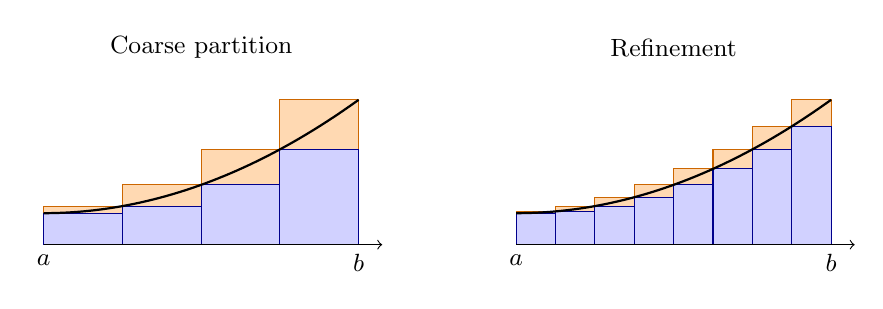
\begin{tikzpicture}[x=1cm,y=1cm,font=\small]
\foreach \shift/\step/\title in {0/1/Coarse partition,6/.5/Refinement}{
\begin{scope}[xshift=\shift cm]
\node at (2,2.5) {\title};
\pgfmathtruncatemacro{\last}{4/\step-1}
\foreach \i in {0,...,\last}{
\pgfmathsetmacro{\a}{\step*\i}
\pgfmathsetmacro{\b}{\a+\step}
\pgfmathsetmacro{\lo}{.4+.09*\a*\a}
\pgfmathsetmacro{\hi}{.4+.09*\b*\b}
\fill[blue!18] (\a,0) rectangle (\b,\lo);
\filldraw[fill=orange!30,draw=orange!80!black] (\a,\lo) rectangle (\b,\hi);
\draw[blue!55!black] (\a,0) rectangle (\b,\lo);
}
\draw[->] (0,0)--(4.3,0);
\draw[thick] plot[domain=0:4,samples=50] (\x,{.4+.09*\x*\x});
\node[below] at (0,0) {$a$};\node[below] at (4,0) {$b$};
\end{scope}}
\end{tikzpicture}
\caption{Blue rectangles give the lower sum; adding the orange bands gives
the upper sum. Inserting cuts raises the lower sum and lowers the upper
sum. The orange area, the Darboux gap, decreases.}
\label{fig:refinement-gap}
\end{figure}
